\documentclass{beamer}
%
% Choose how your presentation looks.
%
% For more themes, color themes and font themes, see:
% http://deic.uab.es/~iblanes/beamer_gallery/index_by_theme.html
%
\mode<presentation>
{
  \usetheme{Hannover}      % or try Darmstadt, Madrid, Warsaw, ...
  \usecolortheme{seagull} % or try albatross, beaver, crane, ...
  \usefonttheme{structurebold}  % or try serif, structurebold, ...
  \setbeamertemplate{navigation symbols}{}
  \setbeamertemplate{caption}[numbered]
} 

\usepackage[german]{babel}
\usepackage[utf8x]{inputenc}

\title[]{Entwicklung eines anwendungsspezifischen Netzwerkprotokolls}
\author{Leonard Petereit\hfill \hspace{0.5cm} Frau Dr. Moor\\ Benedikt Schäfer\hfill \hspace{1cm} Herr Süpke \\ Jan Sommerfeld \hspace{4.25cm} }
\institute{Albert-Schweitzer Gymnasium Erfurt - Spezialschulteil}
\date{27. Juni 2018}

\begin{document}

\begin{frame}
	
  \titlepage
\end{frame}

% Uncomment these lines for an automatically generated outline.
\begin{frame}{Gliederung}

  \tableofcontents
\end{frame}


% Commands to include a figure:
%\begin{figure}
%\includegraphics[width=\textwidth]{your-figure's-file-name}
%\caption{\label{fig:your-figure}Caption goes here.}
%\end{figure}


\section{Technische Grundlagen des Projektes}

\begin{frame}{Technische Grundlagen des Projektes}

\end{frame}

\section{Beschreibung und Zielstellung unserer Arbeit}

\begin{frame}{Beschreibung und Zielstellung der Arbeit}
\begin{figure}
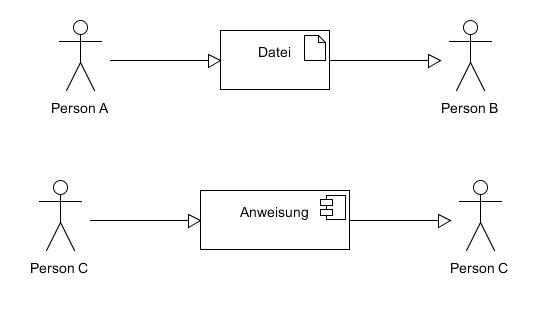
\includegraphics[width=\textwidth]{s1.jpg}

\end{figure}
\end{frame}

\begin{frame}{Beschreibung und Zielstellung der Arbeit}
\begin{figure}
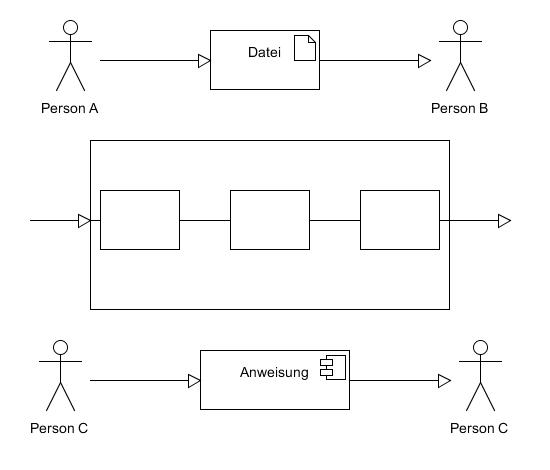
\includegraphics[width=8.5cm]{s2-c.jpg}
\end{figure}
\end{frame}

\begin{frame}{Beschreibung und Zielstellung der Arbeit}
\begin{figure}
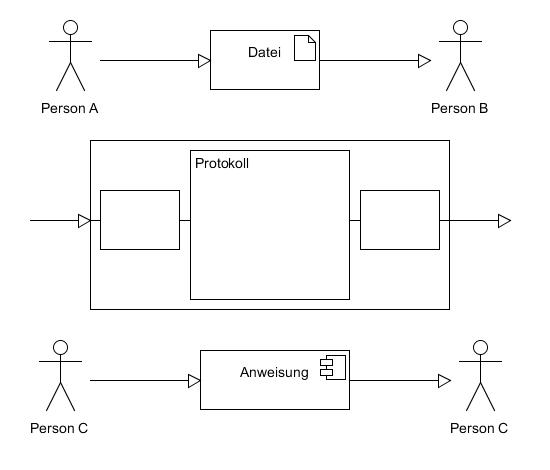
\includegraphics[width=8.5cm]{s3.jpg}
\end{figure}
\end{frame}

\begin{frame}{Beschreibung und Zielstellung der Arbeit}
\begin{figure}
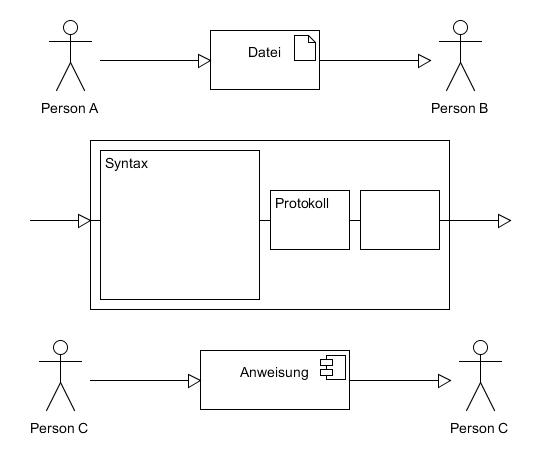
\includegraphics[width=8.5cm]{s4.jpg}
\end{figure}
\end{frame}

\begin{frame}{Beschreibung und Zielstellung der Arbeit}
\begin{figure}
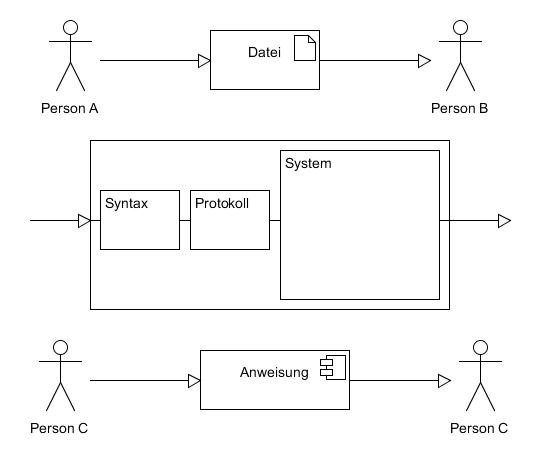
\includegraphics[width=8.5cm]{s5.jpg}
\end{figure}
\end{frame}


\section{Kritische Reflexion des Fortschritts und Gruppenklimas}

\begin{frame}{Kritische Reflexion des Fortschritts und Gruppenklimas}

\end{frame}


\section{Zielstellung für Klasse 12}
\begin{frame}{Zielstellung für Klasse 12}
\pause
\begin{itemize}
\item Entwicklung und Implementierung des UIs und der Syntax
\pause
\item offene Kapitel beenden
\pause
\item Zusammenführung beider Programmteile
\pause
\item Überarbeiten und Überprüfen der Kapitel
\pause
\item evtl. Erweiterung in Verbesserung der UI bzw. Portierung auf Mobilgeräte
\end{itemize}
\end{frame}


\end{document}
